\documentclass{article}

\usepackage{amsmath,amssymb}
\usepackage{graphicx}
\usepackage{subfigure}
\usepackage{multirow}
\usepackage{color}
\usepackage{marginnote}
%\usepackage{longtable}

%\usepackage{color}
%\usepackage{listings}

\usepackage{framed} % PPD
\usepackage{textpos} % PPD

\renewcommand{\baselinestretch}{1}
\renewcommand{\arraystretch}{1.3}

%you may inactive the following four commands, then it will become appearance of book pages

%\setlength{\topmargin}{-0.1in}
%\setlength{\textheight}{8.3in}
%\setlength{\oddsidemargin}{0.1 in}
%\setlength{\textwidth}{6.2 in}

\setlength{\topmargin}{-0.4in}
%\setlength{\topmargin}{-0.1in}
\setlength{\textheight}{9in}
%\setlength{\textheight}{8.3in}
\setlength{\evensidemargin}{-0.4 in}
\setlength{\oddsidemargin}{-0.4 in}
%\setlength{\oddsidemargin}{0.1 in}
\setlength{\textwidth}{7 in}
%\setlength{\textwidth}{6.2 in}

%%%%%%%%%%%%%

\newtheorem{fact}{Fact}
\newtheorem{algorithm}{Algorithm}
\newtheorem{theorem}{Theorem}
\newtheorem{lemma}{Lemma}
\newtheorem{corollary}{Corollary}
\newtheorem{property}{Property}
\newtheorem{definition}{Definition}
\newtheorem{proposition}{Proposition}
\newtheorem{remark}{Remark}
\newtheorem{conjecture}{Conjecture}

\newcommand{\notsim}{{\, \not \sim \,}}

\newcommand{\F}{\ensuremath{\mathbb F}}
\newcommand{\Z}{\ensuremath{\mathbb Z}}
\newcommand{\N}{\ensuremath{\mathbb N}}
\newcommand{\Q}{\ensuremath{\mathbb Q}}
\newcommand{\R}{\ensuremath{\mathbb R}}
\newcommand{\C}{\ensuremath{\mathbb C}}

\newcommand{\done}{\hfill $\Box$ }
\newcommand{\rmap}{\stackrel{\rho}{\leftrightarrow}}
\newcommand{\mys}{\vspace{0.15in}}

\newcommand{\ebu}{{\bf{e}}}
\newcommand{\Abu}{{\bf{A}}}
\newcommand{\Bbu}{{\bf{B}}}

\newcommand{\abu}{{\bf{a}}}
\newcommand{\abuj}{{\bf{a_j}}}
\newcommand{\bbu}{{\bf{b}}}
\newcommand{\vbu}{{\bf{v}}}
\newcommand{\ubu}{{\bf{u}}}
\newcommand{\dbu}{{\bf{d}}}
\newcommand{\tbu}{{\bf{t}}}
\newcommand{\cbu}{{\bf{c}}}
\newcommand{\kbu}{{\bf{k}}}
\newcommand{\hbu}{{\bf{h}}}
\newcommand{\sbu}{{\bf{s}}}
\newcommand{\wbu}{{\bf{w}}}
\newcommand{\xbu}{{\bf{x}}}
\newcommand{\ybu}{{\bf{y}}}
\newcommand{\zbu}{{\bf{z}}}


\newcommand{\corres}{\leftrightarrow}

\newcommand{\zero}{{\bf{0}}}
\newcommand{\one}{{\bf{1}}}
\newcommand{\nodiv}{{\, \not| \,}}
\newcommand{\notequiv}{{\,\not\equiv\, }}

%%%%%%%%%%%%%%

\def\comb#1#2{{#1 \choose #2}}
\newcommand{\ls}[1]
    {\dimen0=\fontdimen6\the\font\lineskip=#1\dimen0
     \advance\lineskip.5\fontdimen5\the\font
     \advance\lineskip-\dimen0
     \lineskiplimit=0.9\lineskip
     \baselineskip=\lineskip
     \advance\baselineskip\dimen0
     \normallineskip\lineskip\normallineskiplimit\lineskiplimit
     \normalbaselineskip\baselineskip
     \ignorespaces}

\def\stir#1#2{\left\{#1 \atop #2 \right\}}
\def\dsum#1#2{#1 \atop #2 }
\def\defn{\stackrel{\triangle}{=}}

%%%%%%%%



\begin{document}

\thispagestyle{plain}
\setcounter{page}{1}

\begin{center}
{\huge {\bf Indian Institute of Technology, Kharagpur}} 

{\LARGE {\em Department of Computer Science and Engineering}}
\vspace{0.4cm}

{\Large \bf Software Engineering (CS 20006), Spring 2015-16} \vspace{0.1cm}

{\large \bf Selection Sort} \vspace{0.1cm}

%{\large \em Req. Spec., and Outline of Analysis, Design, and Testplan} %\vspace{0.3cm}
\end{center}

\hspace{-1cm}

\hspace{-1cm}



You have developed the \texttt{SelectionSort} function to sort an array \texttt{a} of \texttt{nCount} elements in ascending order. Now you need to prepare various white-box tests for the code. For this you would use program analysis techniques and prepare minimal set of test cases for every scenario. 

\begin{framed}
\begin{verbatim}
    void SelectionSort(int a[], unsigned int nCount) { // Sorts by Selection
        unsigned int i, j; // Indices to run over the array

01:     for(i = 0; 
02:         i < nCount; 
03:         ++i) {
04:         unsigned int minLoc = i; // Where the min occurs 
05:         int min = a[minLoc];     // Start a[i] as min 
06:         for(j = i; 
07:             j < nCount; 
08:             ++j) { // Find the min in the rest of the array
09:             if (a[j] < min) {
10:                 minLoc = j;
11:                 min = a[minLoc];
12:             }
13:         } // Inner for loop
14:         a[minLoc] = a[i]; // Swap min with a[i]
15:         a[i] = min;
16:     } // Outer for loop
17:     return;
18: }
\end{verbatim}
\end{framed}


\begin{enumerate}
\item \label{SelectionSort_CFG} Construct the CFG (Control Flow Graph) for \texttt{SelectionSort} using the line numbers as shown. [{\bf 5}]
\begin{framed}
{\bf Answer:}

{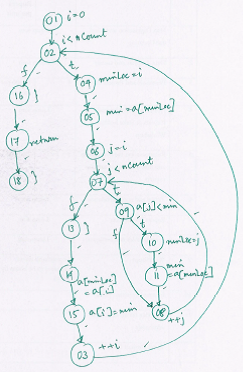
\includegraphics[width=4.5cm]{Images/SelectionSortCFG.png}}
\end{framed}
\newpage
\item \label{SelectionSort_Cyclomatic_Complexity} Compute the cyclomatic complexity of \texttt{SelectionSort} using the CFG in~\ref{SelectionSort_CFG}. [{\bf 2}]
\begin{framed}
{\bf Answer:}

{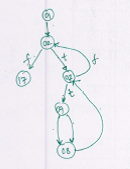
\includegraphics[width=3cm]{Images/CyclomaticComplexity.png}}

Number of nodes $N=18$

Number of Edges $E=10$

Cyclomatic Complexity $V(G) = E - N + 2 = 3$
\end{framed}
\item \label{SelectionSort_LIP} Compute the Linearly Independent Paths (LIP) in~\ref{SelectionSort_CFG}. [{\bf 3}]
\item \label{SelectionSort_LIP_Tests} For every LIP in~\ref{SelectionSort_LIP}, design a test case each that forces the control to trace the LIP. [{\bf 3}]
\item \label{SelectionSort_Block_Coverage} Does tests in~\ref{SelectionSort_LIP_Tests} guarantee 100\% line coverage? Justify or identify an uncovered line. [{\bf 2}]
%\item Justify that 100\% block coverage in~\ref{SelectionSort_Block_Coverage} guarantees 100\% line coverage. [{\bf 2}]
\item Show by a counter example that 100\% block coverage in~\ref{SelectionSort_CFG} may not guarantee 100\% branch coverage. [{\bf 2}]
\item \label{SelectionSort_DEF_USES} Compute the \texttt{DEF} \& \texttt{USES} sets and \texttt{DU}-chains for \texttt{minLoc} and \texttt{min}. Design test cases to cover these \texttt{DU}-chains. [{\bf 2+2=4}]
\item For each of the following mutations (applied separately), check whether the test suite in~\ref{SelectionSort_LIP_Tests} can kill the mutant. If not, design the killer test. [{\bf 2+2=4}]
\begin{itemize}
\item Mutant 1:
\begin{verbatim}
06:         for(j = i;
\end{verbatim}
\ \ \ \ changed to 
\begin{verbatim}
06:         for(j = 0;
\end{verbatim}
\item Mutant 2:
\begin{verbatim}
09:             if (a[j] < min) {
\end{verbatim}
\ \ \ \ changed to 
\begin{verbatim}
09:             if (a[j] > min) {
\end{verbatim}
\end{itemize}

\end{enumerate}

\end{document}
